\documentclass{classrep}
\usepackage[utf8]{inputenc}
\usepackage{color}
\usepackage{makecell}
\usepackage{graphicx}
\usepackage{url}
\usepackage{hyperref}

\studycycle{Informatyka, studia STACJONARNE, I st.}
\coursesemester{VI}

\coursename{Komputerowe systemy rozpoznawania}
\courseyear{2020/2021}

\courseteacher{prof. dr hab. inż. Adam Niewiadomski}
\coursegroup{poniedziałek, 12:00}

\author{
  \studentinfo{Julia Szymańska}{224441} \and
  \studentinfo{Przemysław Zdrzalik}{224466} }

\title{Projekt 1. Klasyfikacja dokumentów tekstowych}
\usepackage{multirow}
\begin{document}
\maketitle


%%%%%%%%%%%%%%%%%%%%%%%%%%%%%%%%%%%%%%%%%%%%%%%%%%%%%%%%%%%%%%%%%%
\section{Cel projektu}

Celem projektu jest stworzenie aplikacji klasyfikującej zadany zbiór danych tekstowych metodą K najbliższych sąsiadów (k-NN). Aplikacja ma za zadanie dokonać ekstrakcji cech na zbiorach tekstów\cite{dane} oraz następnie dokonać ich klasyfikacji.\\


%%%%%%%%%%%%%%%%%%%%%%%%%%%%%%%%%%%%%%%%%%%%%%%%%%%%%%%%%%%%%%%%%%
\section{Klasyfikacja nadzorowana metodą $k$-NN}

Metoda K najbliższych sąsiadów, w skrócie metoda $k$-NN\cite{dane}, jest to algorytm stosowany do klasyfikacji, który nie wymaga etapu uczenia. 
Polega na zaklasyfikowaniu rozpatrywanego elementu do grupy ze zbioru uczącego, gdzie spośród k najbliższych rozpatrywanemu elementowi sąsiadów najwięcej z nich należy do tej grupy. Klasyfikator przyjmuje cztery parametry wejściowe takie jak: warotść k - liczba rozpatrywanych sąsiadów, proporcje podziału zbiorów na zbior uczący i zbiór testowy, zbiór cech, a także metrykę i/lub miarę prawdopodobieństwa. Wynikiem klasyfikacji jest zaklasyfikowanie elementu do jednego ze zbiorów uczących. 


%%%%%%%%%%%%%%%%%%%%%%%%%%%%%%%%%%%%%%%%%%%%%%%%%%%%%%%%%%%%%%%%%%
\subsection{Ekstrakcja cech, wektory cech}

Na zbiorach danych tekstowych należy dokonać ekstrakcji cech, które będą wartościami rzeczywistymi oraz tekstowymi. Dane cechy będą reprezentowały tekst w postaci wektora cech podczas procesu klasyfikacji. Przed dokonaniem ekstrakcji cech, z tekstów usuwane są słowa znajdujące się na stop liście. Teksty ze zbioru danych tekstowych posiadają strukturę: \begin{equation}
  \begin{array}{l}
  <TEXT> \\
\;\;\;\; <TITLE/>\\
\;\;\;\; <AUTHOR/>\\
\;\;\;\; <DATELINE/>\\
 \;\;\;\;<BODY/> \\
</TEXT>
  \end{array}
\end{equation}\\
\begin{enumerate}
  \item Liczba słów - cecha ta oznacza liczbę słów które składają się na pobrany tekst. Cecha ta będzie charakteryzowała długość dokumentu w postaci liczby całkowitej \begin{equation}  c_1 = len \end{equation} gdzie len - liczba słów w tekście.\\
 
 
 \item Data z tagu  \textless Dateline\textgreater\ - Każdy tekst w swoim body posiada tag \textless Dateline\textgreater , w którym znajduje się miasto oraz data podana w postaci miesiąca i dnia. Data będzie konwertowana na wartość liczbową, gdzie liczbą tą będzie numer podanego dnia w ciągu roku, licząc rok tak jakby rok był rokiem przestępnym, przykładowo data 1 marca będzie reprezentowana poprzez wartość 61. Cechę traktujemy jako cechę w postaci liczby całkowitej. Wartość będzie oznaczana poprzez symbol  c\textsubscript{3}.    \\
  \item Lokacja z tagu \textless Dateline\textgreater - jak wyżej. Lokację traktujemy jako cechę tekstową. Wartość będzie oznaczana poprzez symbol  c\textsubscript{4}. \\
  \item Tytuł z tagu \textless Title\textgreater - Każdy tekst w swoim body posiada tag \textless Title\textgreater. Tytuł traktujemy jako cechę tekstową. Wartość będzie oznaczana poprzez symbol  c\textsubscript{5}.\\
  \item Autor z tagu \textless Author\textgreater - Większość tekstów w swoim body posiada tag \textless Author\textgreater. Autora traktujemy jako cechę tekstową. Wartość będzie oznaczana poprzez symbol  c\textsubscript{6}.\\
  \item Najczęściej występująca nazwa kraju - wybieramy najczęściej występującą w analizowanym tekście nazwę kraju. Nazwy krajów pobieramy z dołączonego pliku all-places-strings.lc, przykładowo krajem występującym w pliku jest 'albania'.Nazwę kraju traktujemy jako cechę tekstową.Wartość będzie oznaczana poprzez symbol  c\textsubscript{7}.\\
  \item Zbiór występujących słów kluczowych. Za słowa kluczowe przyjmujemy słowa znajdujące się w dołączonych plikach o rozszerzeniach .lc.txt. Cechę traktujemy jako cechę tekstową.  \begin{equation}  c_8 : c_8 \in N \cap t \end{equation} gdzie N - zbiór wszystkich słów kluczowych, t - zbiór słów należących do tekstu\\
  \item Liczba wystąpień słów kluczowych - traktujemy jako cechę w postaci liczby całkowitej.\begin{equation}  c_9 = | c_8 | \end{equation} gdzie c\textsubscript{8} - zbiór występujących słów kluczowych\\
  \item Nasycenie tekstu ilością słów kluczowych - traktujemy jako cechę w postaci liczby zmienno przecinkowej.  \begin{equation} c_{10} = c_9 / c_1 \end{equation}  gdzie c\textsubscript{9} - liczba wystąpień słów kluczowych w tekscie, c\textsubscript{1} - liczba słów w tekście\\
  \item Najczęściej występujące słowo kluczowe - wybieramy najczęściej występujące w analizowanym tekście słowo kluczowe. Cechę traktujemy jako cechę tekstową. Wartość będzie oznaczana poprzez symbol  c\textsubscript{11}.\\
  \item Liczba unikatowych słów - zliczamy liczbę unikatowych słów, to znaczy występujących dokładnie raz w analizowanym tekście. Cechę traktujemy jako cechę w postaci liczby całkowitej. Wartość będzie oznaczana poprzez symbol  c\textsubscript{12}.\\
\end{enumerate}

\ \\ \\
Wektor cech będzie reprezentowany w postaci: 

\begin{equation} w = [c_1, c_2, c_3, c_4, c_5, c_6, c_7, c_8, c_9, c_{10}, c_{11}] \end{equation}


%%%%%%%%%%%%%%%%%%%%%%%%%%%%%%%%%%%%%%%%%%%%%%%%%%%%%%%%%%%%%%%%%%
\subsection{Miary jakości klasyfikacji} 

W celu określenia jakości wykonanej klasyfikacji korzystamy z czterech miar jakości klasyfikacji. Aby obliczyć każdą z miar tworzymy tablicę pomyłek, inaczej macierz błędu \cite{tablica}. Tablica składa się z dwóch wierszy i dwóch kolumn, gdzie wiersze to klasy predykowane, a kolumny to klasy rzeczywiste. Dane oznaczone jako dane pozytywne i negatywne poddawane są klasyfikacji, która przypisuje im predykowaną klasę pozytywną bądź negatywną.\\

\begin{table}[h!]
\begin{tabular}{l|l|c|c|c}
\multicolumn{2}{c}{}&\multicolumn{2}{c}{Klasa rzeczywista}&\\
\cline{3-4}
\multicolumn{2}{c|}{}&Pozytywna&Negatywna&\multicolumn{1}{c}{}\\
\cline{2-4}
\multirow{2}{*}{\thead{Klasa\\ predykowana} }& Pozytywna&  \thead{prawdziwie\\ pozytywna (TP)}
 & \thead{fałszywie\\ pozytywna (FP)} \\
\cline{2-4}
& Negatywna & \thead{fałszywie\\ negatywna (FN)} & \thead{prawdziwie\\ negatywna (TN)} \\
\cline{2-4}
\end{tabular}
 \caption{Wzór tablicy pomyłek\cite{tablica}.}
\end{table}

We wzorach zostały użyte oznaczenia:
\begin{itemize}
\item TP - liczba poprawnie zaklasyfikowanych tekstów rozpatrywanej klasy 
\item TN - liczba poprawnie zaklasyfikowanych tekstów pozostałych klas
\item FP - liczba tekstów pozostałych klas zaklasyfikowanych do rozpatrywanej klasy
\item FN - liczba tekstów rozpatrywanej klasy zaklasyfikowanych do pozostałych klas
\end{itemize}

\ \\ \\ 
Stosowane miary jakości klasyfikacji:\\
\begin{itemize}
  \item Dokładność (ang. accuracy), ACC  - jest to stosunek poprawnie zaklasyfikowanych tekstów do wszystkich klasyfikowanych tekstów.
 \begin{equation}ACC = \frac{TP + TN}{TP + TN + FP + FN} \end{equation}
 \item Precyzja (ang. precision), PPV  - jest to stopień zgodności wyników uzyskanych w określonych warunkach z wielokrotnych pomiarów. Precyzja to stosunek liczby poprawnie zaklasyfikowanych tekstów rozpatrywanej klasy do liczby wszystkich tekstów zaklasyfikowanych do rozpatrywanej klasy . 
 \begin{equation} PPV =  \frac{TP} {TP+FP} \end{equation}
\item Czułość (ang. recall), TPR  - jest to stosunek liczby poprawnie zaklasyfikowanych tekstów do rozpatrywanej klasy do liczby tekstów z rozpatrywanej klasy. 
 \begin{equation}   TPR = \frac{TP}{TP + FN} \end{equation}
\item Miara F1 - średnia harmoniczna miar Precyzja i Czułość. 
\begin{equation}   F1 = \frac{2}{\frac{1}{PPV} + \frac{1}{TPR}} \end{equation}
\end{itemize}


%%%%%%%%%%%%%%%%%%%%%%%%%%%%%%%%%%%%%%%%%%%%%%%%%%%%%%%%%%%%%%%%%%
\section{Klasyfikacja z użyciem metryk i miar podobieństwa tekstów}

W procesie klasyfikacji możliwe jest wykorzystanie jednej z trzech metryk: metryka Euklidesowa, metryka Czebyszewa, metryka Uliczna. Metryki służą obliczeniu odległości pomiędzy dwoma wektora o dowolnym rozmiarze.\\\\ Metryka Eukliedesowa\cite{dane} jest opisana wzorem: 
\begin{equation} d(x, y) = \sqrt{(y_1 - x_1)^2 + ... + (y_n - x_n)^2}  \end{equation}
gdzie: d(x, y) - odległość pomiędzy wektorem x i y; x, y - wektory o tym samym rozmiarze; n - rozmiar wektorów x i y;  x\textsubscript{n}, y\textsubscript{n} - składowe wektora. 
\\\\
Metryka Czebyszewa\cite{dane} jest opisana wzorem: 
\begin{equation} d(x, y) = max(|y_i - x_i|) \end{equation}
gdzie: d(x, y) - odległość pomiędzy wektorem x i y; x, y - wektory o tym samym rozmiarze; n - rozmiar wektorów x i y;  x\textsubscript{i}, y\textsubscript{i} - i-ta składowa wektora;
\\\\
Metryka Uliczna\cite{dane} jest opisana wzorem: 
\begin{equation} d(x, y) = \sum_{i = 1}^{n} |x_i - y_i| \end{equation}
gdzie: d(x, y) - odległość pomiędzy wektorem x i y; x, y - wektory o tym samym rozmiarze; n - rozmiar wektorów x i y;  x\textsubscript{n}, y\textsubscript{n} - składowe wektora. 
\\\\
By móc obliczyć odległość pomiędzy wektorami cech zadanych tekstów, należy wcześniej skorzystać z miar podobieństwa tekstu by zamienić cechy o wartościach tekstowcyh na liczby w wektorach. W programie zostało użyte podobieństwo kosinusowe\cite{wyklad}. Należy utworzyć po jedym wektorze dla cechy o wartości tekstowej dla każdego z dwóch rozpatrywanych tekstów - x = \{ x\textsubscript{1}, x\textsubscript{2}, ... , x\textsubscript{n} \},  y = \{ y\textsubscript{1}, y\textsubscript{2}, ... , y\textsubscript{n} \}, gdzie x\textsubscript{n}, y\textsubscript{n}  to liczba wystąpień n-tego słowa, ze zbioru wszystkich słów występujących w obu wektorów, w zadanej cesze tekstowej wektora cech. Dla tak utworzonych wektrów liczony jest kosinus kąta pomiędzy nimi ze wzoru:
\begin{equation} r_{cos} = \frac{\sum_{i = 1}^{n} x y}{\sqrt{\sum_{i = 1}^{n} x^2}\sqrt{\sum_{i = 1}^{n} y^2}} \end{equation}
gdzie r\textsubscript{cos} - to cos kąta pomiędzy wektorem x i y; x, y - rozpatrywane wektory; n - długość wektora.
\ \\ \\ 


Wstępna klasyfikacja na ograniczonym zbiorze tekstów została przeprowadzona dla trzech różnych zestawów parametrów wejściowych. \newline
Parametry wejściowe dla pierwszej klasyfikacji wstępnej:
 
\begin{table}[h!]
\caption{Parametry wejściowe dla pierwszej wstępnej klasyfikacji. }
\centering
\vspace{0.1cm}
 \begin{tabular}{c c c c}
    \textbf{K} & \textbf{Metryka}   & \textbf{Procent zbioru trenującego}  & \textbf{Wybrane cechy}   \\
\hline
5 & Czebyszewa & 80\% & Wszysktie cechy \\
\end {tabular}
\label {Parametry wejściowe dla pierwszej wstępnej klasyfikacji. }
\end{table}
\newpage

Wstępne wyniki miary Accuracy dla pierwszej klasyfikacji wstępnej:

\begin{table}[h!]
\caption{Wstępne wyniki miary Accuracy dla pierwszej klasyfikacji wstępnej.}
\centering
\vspace{0.1cm}
 \begin{tabular}{c c c c c c}

    \textbf{Liczba tekstów} &  \makecell{\textbf{Liczba poprawnie} \\\textbf{sklasyfikowanych tekstów}}  & \textbf{Accuracy}\\
\hline
394 & 230 & 0,58\\

\end {tabular}
\label {Wstępne wyniki miary Accuracy dla pierwszej klasyfikacji wstępnej.}
\end{table}


Parametry wejściowe dla drugiej klasyfikacji wstępnej:
 
\begin{table}[h!]
\caption{Parametry wejściowe dla drugiej wstępnej klasyfikacji. }
\centering
\vspace{0.1cm}
 \begin{tabular}{c c c c}
    \textbf{K} & \textbf{Metryka}   & \textbf{Procent zbioru trenującego}  & \textbf{Wybrane cechy}   \\
\hline
3 & Euklidesowa & 95\% &  \makecell{1. Lokalizacja \\2. Tytuł\\3. Najczęściej występująca\\nazwa państwa\\4. Kluczowe słowa}\\
\end {tabular}
\label {Parametry wejściowe dla drugiej wstępnej klasyfikacji. }
\end{table}

Wstępne wyniki miary Accuracy dla drugiej klasyfikacji wstępnej:

\begin{table}[h!]
\caption{Wstępne wyniki miary Accuracy dla drugiej klasyfikacji wstępnej.}
\centering
\vspace{0.1cm}
 \begin{tabular}{c c c c c c}

    \textbf{Liczba tekstów} &\makecell{\textbf{Liczba poprawnie} \\\textbf{sklasyfikowanych tekstów}} & \textbf{Accuracy}\\
\hline
394 & 295 & 0,75\\

\end {tabular}
\label {Wstępne wyniki miary Accuracy dla drugiej klasyfikacji wstępnej.}
\end{table}


Parametry wejściowe dla trzeciej klasyfikacji wstępnej:
 
\begin{table}[h!]
\caption{Parametry wejściowe dla trzeciej wstępnej klasyfikacji. }
\centering
\vspace{0.1cm}
 \begin{tabular}{c c c c}
    \textbf{K} & \textbf{Metryka}   & \textbf{Procent zbioru trenującego}  & \textbf{Wybrane cechy}   \\
\hline
9 & Uliczna & 73\% &  \makecell{1. Kluczowe słowa \\2. Liczba kluczowych słów\\3. Nasycenie tekstu\\słowani kluczowymi\\4. Najczęściej występujące \\słowani kluczowymi}\\
\end {tabular}
\label {Parametry wejściowe dla trzeciej wstępnej klasyfikacji. }
\end{table}

Wstępne wyniki miary Accuracy dla trzeciej klasyfikacji wstępnej:

\begin{table}[h!]
\caption{Wstępne wyniki miary Accuracy dla trzeciej klasyfikacji wstępnej.}
\centering
\vspace{0.1cm}
 \begin{tabular}{c c c c c c}

    \textbf{Liczba tekstów} &\makecell{\textbf{Liczba poprawnie} \\\textbf{sklasyfikowanych tekstów}} & \textbf{Accuracy}\\
\hline
394 & 236 & 0,60\\

\end {tabular}
\label {Wstępne wyniki miary Accuracy dla trzeciej klasyfikacji wstępnej.}
\end{table}


%%%%%%%%%%%%%%%%%%%%%%%%%%%%%%%%%%%%%%%%%%%%%%%%%%%%%%%%%%%%%%%%%%
\section{Budowa aplikacji}
\subsection{Diagramy UML}

Aplikacja będzie składała się z dwóch modułów: z modułu ekstrakcji cech oraz z modułu klasyfikacji. Moduł ekstrakcji wczytuje pliki z treścią artykułów. Następnie tworzone są obiekty artykułów. Dla każdego obiektu usuwane są słowa ze stop listy oraz kolejno tworzone są wektory cech artykułów. 

\begin{figure}[h!]
 \centering
 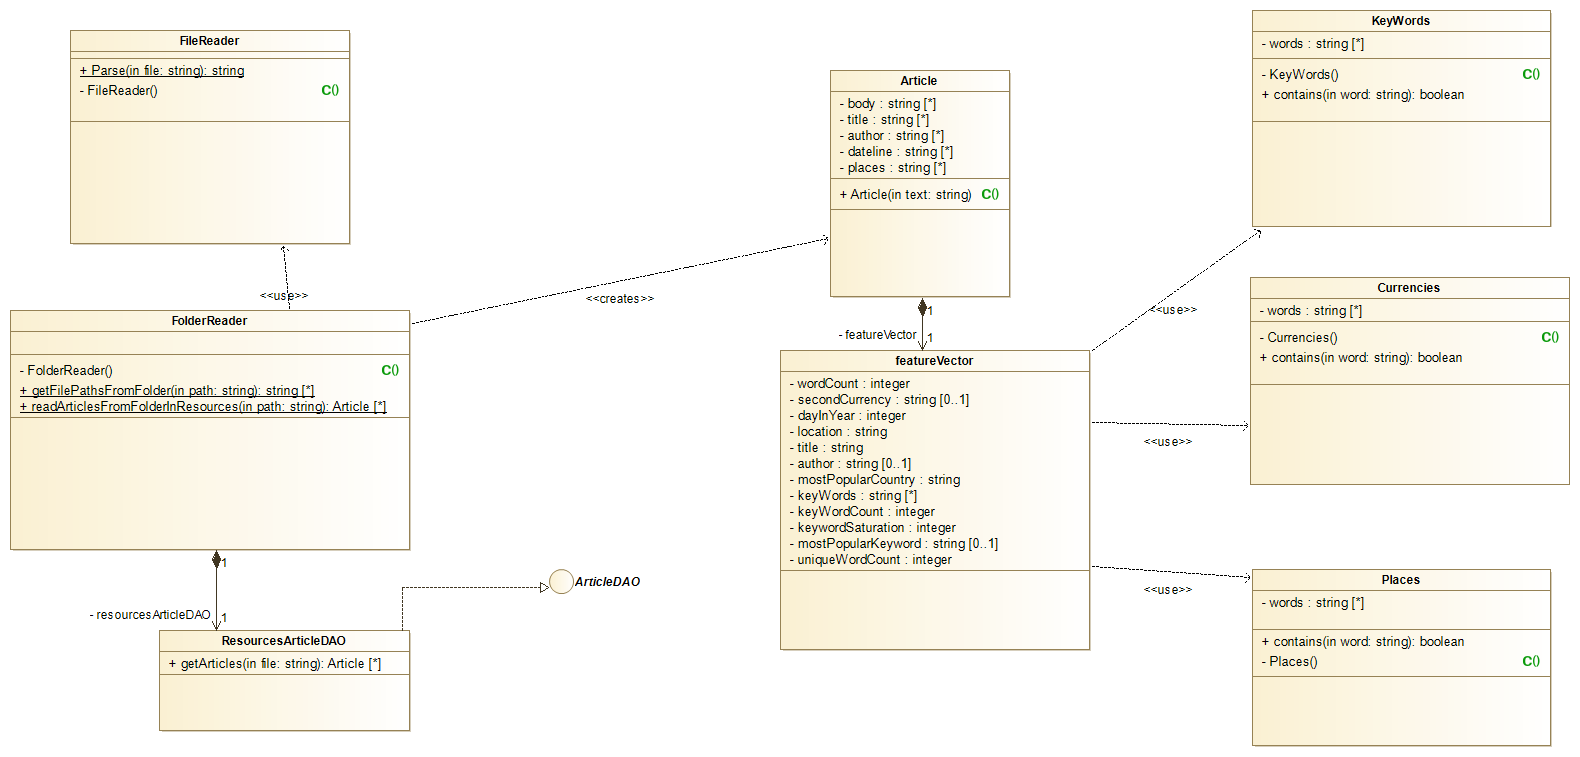
\includegraphics[width=14cm]{Ekstrakcja.png}
 \vspace{-0.3cm}
 \caption{Diagram klas modułu ekstrakcji cech. }
 \label{rysunek do eksperymentu 1 wariantu 1}
\end{figure}
\newpage

Moduł klasyfikacji oblicza odległości pomiędzy artykułem zadanym a każdym z artykułów ze zbioru trenującego za pomocą jednej z zadanych metryk \cite{dane} : metryki Euklidesowej, metryki Ulicznej, metryki Czebyszewa. Dla cech zapisanych w postaci tekstowej ich odległość jest obliczana za pomocą podobieństwa kosinusowego. W ten sposób tworzone są pary zawierające artykuł i odleglość od zadanego artykułu. Następnie znajdowanych jest k najbliższych sąsiadów dla zadanego artykułu, gdzie poprzez słowo sąsiad rozumiemy artykuł ze zbioru trenującego. Ostatecznie artykuł jest klasyfikowany do klasy, której obiekty najczęściej wystąpiły wśród k najbliższych sąsiadów. 

\begin{figure}[h!]
 \centering
 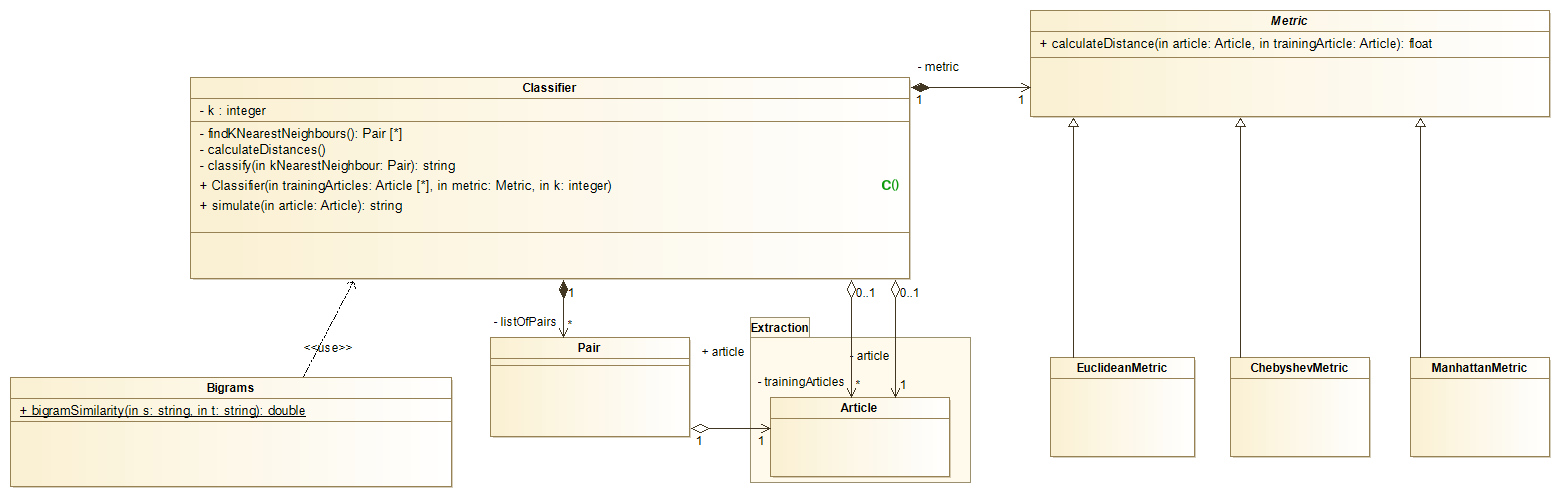
\includegraphics[width=14cm]{Klasyfikator.png}
 \vspace{-0.3cm}
 \caption{Diagram klas modułu klasyfikacji. }
 \label{rysunek do eksperymentu 1 wariantu 1}
\end{figure}

\newpage


%%%%%%%%%%%%%%%%%%%%%%%%%%%%%%%%%%%%%%%%%%%%%%%%%%%%%%%%%%%%%%%%%%
\subsection{Prezentacja wyników, interfejs użytkownika} 

Po uruchomieniu programu użytkownik proszony jest o podanie poprzez konsolę kolejnych parametrów klasyfikacji. Na początku użytkownik podaje wartość parametru k, następnie wybiera jedną z trzech metryk, kolejno podawany jest procent zbioru treningowego w stosunku do zbioru wszystkich tekstów oraz użytkownik może podać cechy tesktów do klasyfikacji. Wybór parametrów w konsoli prezentuje się:

\begin{figure}[h!]
 \centering
 \includegraphics[width=14cm]{Wybor.png}
 \vspace{-0.3cm}
 \caption{Wybór parametrów klasyfikacji przez użytkownika. }
 \label{Wybór parametrów klasyfikacji przez użytkownika. }
\end{figure}

\newpage
Po wprowadzeniu przez użytkownika wszystkich parametrów klasyfikacji, rozpoczynane jest wczytywanie danych oraz wykonanie klasyfikacji. 
\begin{figure}[h!]
 \centering
 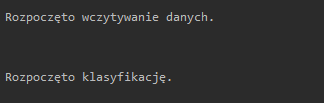
\includegraphics[width=14cm]{srodek.png}
 \vspace{-0.3cm}
 \caption{Wczytywanie danych i klasyfikacja.}
 \label{Wczytywanie danych i klasyfikacja.}
\end{figure}




Po wykonanej klasyfikacji na konsoli wyświetlane są obliczone parametry dla poszczególnych klas klasyfikacji oraz wyliczone parametry dla całego zbioru dokumentów. Dla poszczególnych klas klasyfikacji do obliczonych parametrów zaliczamy liczbę tekstów klasy, liczbę poprawnie zaklasyfikowanych tekstów do rozpatrywanej klasy, liczbę tekstów innych klas zaklasfyfikowanych do rozpatrywanej klasy oraz miary jakości: Precision, Recall, F1. 
\begin{figure}[h!]
 \centering
 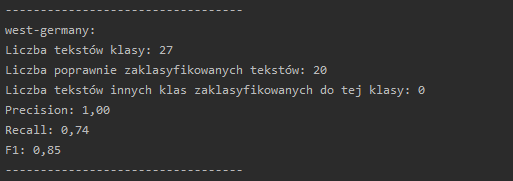
\includegraphics[width=14cm]{wynik_dla _klasy.png}
 \vspace{-0.3cm}
 \caption{Wynik klasyfikacji dla pojedyńczej klasy klasyfikacji - klasa west-germany.}
 \label{Wynik klasyfikacji.}
\end{figure}

Dla całego zbioru dokumentów do obliczonych parametrów zaliczamy liczbę tekstów testowych, liczbę poprawnie zaklasyfikowanych tekstów oraz miary jakości: Accuracy, Precision, Recall, F1. 
  
\begin{figure}[h!]
 \centering
 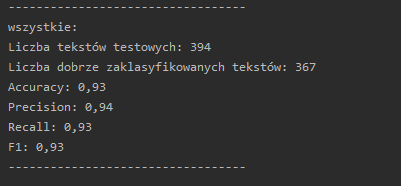
\includegraphics[width=14cm]{wynik.png}
 \vspace{-0.3cm}
 \caption{Wynik klasyfikacji dla całego zbioru dokumentów.}
 \label{Wynik klasyfikacji.}
\end{figure}
\newpage

Do uruchomienia programu wymagana jest wersja Javy: 11. 



%%%%%%%%%%%%%%%%%%%%%%%%%%%%%%%%%%%%%%%%%%%%%%%%%%%%%%%%%%%%%%%%%%
\section{Wyniki klasyfikacji dla różnych parametrów wejściowych}

Eksperymenty zostały rozpoczęte od porównania wyników klasyfikacji dla różnych wartości parametru k.
W tym celu przyjęliśmy nastepujące parametry:
 
\begin{table}[h!]
\caption{Parametry wejściowe dla eksperymentu porównującego różne wartości parametru k. }
\centering
\vspace{0.1cm}
 \begin{tabular}{c c c c}
    \textbf{K} & \textbf{Metryka}   & \textbf{Procent zbioru trenującego}  & \textbf{Wybrane cechy}   \\
\hline
- & Euklidesowa & 80\% &  Wszystkie cechy\\
\end {tabular}
\label {Parametry wejściowe dla eksperymentu porównującego różne wartości parametru k. }
\end{table}

\newpage
\begin{table}[h!]
\caption{Wyniki klasyfikacji dla różnych wartości parametru k.}
\centering
\vspace{0.1cm}
 \begin{tabular}{c c c c c c c c c c c}

    \textbf{K} & \textbf{1}   & \textbf{2}  & \textbf{3}  & \textbf{4}  & \textbf{5} & \textbf{7}   & \textbf{10}  & \textbf{20}  & \textbf{50}  & \textbf{100} \\

\hline
West-germany Precission 	& 0,23 & NaN & 0,00 & NaN  & NaN & NaN  & NaN & NaN & NaN  & NaN\\
West-germany Recall 		& 0,11 & 0,00 & 0,00 & 0,00 & 0,00 & 0,00 & 0,00 & 0,00 & 0,00 & 0,00\\
West-germany F1		& 0,15 & NaN & 0,00 & NaN  & NaN & NaN  & NaN & NaN & NaN  & NaN \\
\hline
Usa Precission 			& 0,63 & 0,61 & 0,61 & 0,62 & 0,61 & 0,61 & 0,61 & 0,61 & 0,61 & 0,61 \\
Usa Recall				& 0,84 & 0,95 & 0,96 & 0,98 & 1,00 & 1,00 & 1,00 & 1,00 & 1,00 & 1,00 \\
Usa F1			 	& 0,72 & 0,75 & 0,74 & 0,76 & 0,76 & 0,76 & 0,76 & 0,76 & 0,76 & 0,76 \\
\hline
France Precission 		& 0,00 & NaN & 1,00 & NaN  & NaN  & NaN & NaN & NaN  & NaN & NaN \\
France Recall 			& 0,00 & 0,00 & 0,09 & 0,00 & 0,00 & 0,00 & 0,00 & 0,00 & 0,00 & 0,00 \\
France F1 				& 0,00 & NaN & 0,17 & NaN  & NaN  & NaN & NaN & NaN  & NaN & NaN\\
\hline
Uk Precission 			& 0,24 & 0,75 & 0,00 & 0,40 & NaN  & NaN & NaN & NaN  & NaN & NaN\\
Uk Recall 				& 0,24 & 0,09 & 0,00 & 0,06 & 0,00 & 0,00 & 0,00 & 0,00 & 0,00 & 0,00\\
Uk F1 				& 0,24 & 0,16 & 0,00 & 0,11 & NaN  & NaN & NaN & NaN  & NaN & NaN \\
\hline
Canada Precission		& 0,10 & 0,00 & 0,00 & 0,50 & 0,00 & 0,00 & NaN & NaN  & NaN & NaN\\
Canada Recall 			& 0,03 & 0,00 & 0,00 & 0,03 & 0,00 & 0,00 & 0,00 & 0,00 & 0,00 & 0,00 \\
Canada F1 			& 0,04 & 0,00 & 0,00 & 0,05 & 0,00 & 0,00 & NaN &NaN  & NaN & NaN \\
\hline
Japan Precission 		& 0,07 & 0,00 & NaN & 0,50 & NaN  & NaN & NaN & NaN & NaN & NaN \\
Japan Recall 			& 0,02 & 0,00 & 0,00 & 0,05 & 0,00 & 0,00 & 0,00 & 0,00 & 0,00 & 0,00 \\
Japan F1 				& 0,04 & 0,00 & NaN & 0,09 & NaN  & NaN & NaN & NaN & NaN & NaN\\
\hline
Accuracy 				& 0,55 & 0,59 & 0,59 & 0,61 & 0,61 & 0,61 & 0,61 & 0,61 & 0,61 & 0,61 \\
Precission 				& 0,44 & 0,44 & 0,40 & 0,52 & 0,37  & 0,37 & 0,37 &  0,37  & 0,37 & 0,37\\
Recall 				& 0,55 & 0,59 & 0,59 & 0,61 & 0,61 & 0,61 & 0,61 & 0,61 & 0,61 & 0,61  \\
F1 					& 0,48 & 0,47 & 0,46 & 0,49 & 0,46 & 0,46 & 0,46 & 0,46 & 0,46 & 0,46\\

\end {tabular}
\label {Wyniki klasyfikacji dla różnych wartości parametru k.}
\end{table}

Różne wartości parametru k nie mają znacznego znaczenia dla dokładności klasyfikacji. Najgorszy wynik był dla wartości parametru 1. Od wartości k równej 5 wszystkie obiekty zostały zaklasyfikowane do klasy USA, co możemy odczytać z wartości NaN przy obliczaniu precyzji. Wartość taka pojawia się przy dzieleniu przez 0, co oznacza że nie istniał taki obiekt który zostałby sklasyfikowany do danej klasy. \\



%%%%%%%%%%%%%%%%%%%%%%%%%%%%%%%%%%%%%%%%%%%%%%%%%%%%%%%%%%%%%%%%%%
Następnym eksperymentem jest wykonanie klasyfikacji dla różnych metryk. Pozostałe parametry pozostają niezmienne.\\

Wybrane parametry przedstawione są w poniższej tabeli:
 
\begin{table}[h!]
\caption{Parametry wejściowe dla eksperymentu porównującego różne metryki. }
\centering
\vspace{0.1cm}
 \begin{tabular}{c c c c}
    \textbf{K} & \textbf{Metryka}   & \textbf{Procent zbioru trenującego}  & \textbf{Wybrane cechy}   \\
\hline
6 & - & 90\% &  Wszystkie cechy\\
\end {tabular}
\label {Parametry wejściowe dla eksperymentu porównującego różne metryki. }
\end{table}

\newpage
\begin{table}[h!]
\caption{Wyniki klasyfikacji dla różnych metryk.}
\centering
\vspace{0.1cm}
 \begin{tabular}{c c c c}

    \textbf{Metryka} & \textbf{Euklidesowa}   & \textbf{Czebyszewa}  & \textbf{Uliczna}  \\

\hline
West-germany Precission 	& 0,25 & 0,00 & 0,20 \\
West-germany Recall 		& 0,04 & 0,00 & 0,04 \\
West-germany F1		& 0,06 & 0,00 & 0,06 \\
\hline
Usa Precission 			& 0,61 & 0,61 & 0,62 \\
Usa Recall				& 0,98 & 0,98 & 0,99 \\
Usa F1			 	& 0,75 & 0,76 & 0,76 \\
\hline
France Precission 		& NaN & NaN & NaN \\
France Recall 			& 0,00 & 0,00 & 0,00 \\
France F1 				& NaN & NaN & NaN \\
\hline
Uk Precission 			& 0,00 & 0,00 & 0,00 \\
Uk Recall 				& 0,00 & 0,00 & 0,00 \\
Uk F1 				& 0,00 & 0,00 & 0,00 \\
\hline
Canada Precission		& 0,00 & 0,00 & NaN \\
Canada Recall 			& 0,00 & 0,00 & 0,00 \\
Canada F1 			& 0,00 & 0,00 & NaN \\
\hline
Japan Precission 		& 0,67 & 0,50 & 1,00 \\
Japan Recall 			& 0,05 & 0,02 & 0,05 \\
Japan F1 				& 0,09 & 0,04 & 0,09 \\
\hline
Accuracy 				& 0,60 & 0,60 & 0,61 \\
Precission 				& 0,47 & 0,43 & 0,50 \\
Recall 				& 0,60 & 0,60 & 0,61 \\
F1 					& 0,52 & 0,50 & 0,55 \\

\end {tabular}
\label {Wyniki klasyfikacji dla różnych metryk.}
\end{table}


Metryki uzyskały zbliżone wyniki, spośród nich najlepszą okazała się metryka Uliczna, drugą najlepszą metryką okazała się Euklidesowa. \\



%%%%%%%%%%%%%%%%%%%%%%%%%%%%%%%%%%%%%%%%%%%%%%%%%%%%%%%%%%%%%%%%%%
Następnym eksperymentem jest wykonanie klasyfikacji dla różnych podzbiorów cech. Pozostałe parametry pozostają niezmienne. W tym celu wybieramy sześć różnych zestawów cech. 

\begin{enumerate}
\item Autor z tagu Author, lokalizacja z tagu Dateline, tytuł z tagu Title, zbiór słów kluczowych
\item Liczba słów, Autor z tagu Author, liczba unikalnych słów, data z tagu Dateline, najczęściej występująca nazwa kraju
\item Lokalizacja z tagu Dateline, tytuł z tagu Title, zbiór słów kluczowych, najczęściej występujące słowo kluczowe
\item Lokalizacja z tagu Dateline, tytuł z tagu Title
\item Lokalizacja z tagu Dateline
\item Tytuł z tagu Title
\end{enumerate}

Parametry wejściowe dla eksperymentu porównującego różne podzbiorów cech:
 
\begin{table}[h!]
\caption{Parametry wejściowe dla eksperymentu porównującego różne podzbiorów cech. }
\centering
\vspace{0.1cm}
 \begin{tabular}{c c c c}
    \textbf{K} & \textbf{Metryka}   & \textbf{Procent zbioru trenującego}  & \textbf{Wybrane cechy}   \\
\hline
6 & Euklidesa & 90 & -\\
\end {tabular}
\label {Parametry wejściowe dla eksperymentu porównującego różne podzbiorów cech. }
\end{table}

\newpage
\begin{table}[h!]
\caption{Wyniki klasyfikacji dla różnych podzbiorów cech.}
\centering
\vspace{0.1cm}
 \begin{tabular}{c c c c c c c}

    \makecell{\textbf{Wyrbany numer} \\\textbf{zestawu cech}} & \textbf{1} & \textbf{2}  & \textbf{3}  & \textbf{4}  & \textbf{5} & \textbf{6}\\

\hline
West-germany Precission 	& 1,00 & 0,20 & 1,00 & 1,00 & 1,00 & 1,00\\
West-germany Recall 		& 0,81 & 0,04 & 0,78 & 0,89 & 0,96 & 0,26\\
West-germany F1		& 0,90 & 0,06 & 0,88 & 0,94 & 0,98 & 0,41\\
\hline
Usa Precission 			& 0,87 & 0,62 & 0,87 & 0,94 & 0,93 & 0,72\\
Usa Recall				& 1,00 & 0,98 & 1,00 & 1,00 & 1,00 & 0,99\\
Usa F1			 	& 0,93 & 0,75 & 0,93 & 0,97 & 0,96 & 0,83\\
\hline
France Precission 		& 1,00 & Nan & 1,00 & 1,00 & 1,00 & 1,00\\
France Recall 			& 0,64 & 0,00 & 0,64 & 1,00 & 1,00 & 0,36\\
France F1 				& 0,78 & Nan & 0,78 & 1,00 & 1,00 & 0,53\\
\hline
Uk Precission 			& 1,00 & 0,33 & 0,94 & 1,00 & 1,00 & 0,67\\
Uk Recall 				& 0,72 & 0,03 & 0,91 & 0,97 & 0,97 & 0,30\\
Uk F1 				& 0,84 & 0,06 & 0,92 & 0,98 & 0,98 & 0,42\\
\hline
Canada Precission		& 1,00 & 0,00 & 1,00 & 0,97 & 1,00 & 0,50\\
Canada Recall 			& 0,72 & 0,00 & 0,67 & 0,82 & 0,82 & 0,13\\
Canada F1 			& 0,84 & 0,00 & 0,80 & 0,89 & 0,90 & 0,20\\
\hline
Japan Precission 		& 1,00 & 1,00 & 1,00 & 1,00 & 1,00 & 0,96\\
Japan Recall 			& 0,67 & 0,05 & 0,72 & 0,91 & 0,79 & 0,60\\
Japan F1 				& 0,81 & 0,09 & 0,84 & 0,95 & 0,88 & 0,74\\
\hline
Accuracy 				& 0,91 & 0,61 & 0,90 & 0,96 & 0,95 & 0,74\\
Precission 				& 0,92 & 0,53 & 0,92 & 0,96 & 0,96 & 0,75\\
Recall 				& 0,91 & 0,61 & 0,90 & 0,96 & 0,95 & 0,74\\
F1 					& 0,90 & 0,48 & 0,90 & 0,96 & 0,95 & 0,69\\

\end {tabular}
\label {Wyniki klasyfikacji dla różnych podzbiorów cech.}
\end{table}


Po porównaniu zestawów cech odkryliśmy, że najlepszą z cech jest Lokalizacja z tagu dateline. Korzystając tylko z tej jednej cechy uzyskaliśmy prawie najlepsze wyniki, które bardzo nieznacznie poprawiło jedynie dodanie do tej cechy cechy Tytułu z tagu Title. Sam tytuł z tagu Title też dał dobre wyniki klasyfikacji, jednak nie tak dobre jak lokalizacja.  Dodawanie innych cech do zestawu tych dwu cech pogarszało wyniki.  \\


%%%%%%%%%%%%%%%%%%%%%%%%%%%%%%%%%%%%%%%%%%%%%%%%%%%%%%%%%%%%%%%%%%


Ostatnim eksperymentem jest wykonanie klasyfikacji dla różnych wartości proporcji podziału zbioru. Pozostałe parametry pozostają niezmienne.\\ 
Wybrane parametry przedstawione są w poniższej tabeli:
 
\begin{table}[h!]
\caption{Parametry wejściowe dla eksperymentu porównującego różne wartości proporcji podziału zbioru. }
\centering
\vspace{0.1cm}
 \begin{tabular}{c c c c}
    \textbf{K} & \textbf{Metryka}   & \textbf{Procent zbioru trenującego}  & \textbf{Wybrane cechy}   \\
\hline
6 & Uliczna & - &  \makecell{ Lokalizacja z tagu Dateline \\Tytuł z tagu Title}\\
\end {tabular}
\label {Parametry wejściowe dla eksperymentu porównującego różne wartości proporcji podziału zbioru. }
\end{table}

\newpage
\begin{table}[h!]
\caption{Wyniki klasyfikacji dla różnych wartości proporcji podziału zbioru.}
\centering
\vspace{0.1cm}
 \begin{tabular}{c c c c c c}

    \textbf{Proporcje} & \textbf{10}   & \textbf{25}  & \textbf{50}  & \textbf{70}  & \textbf{95}\\

\hline
West-germany Precission 	& NaN & 1,00 & 1,00 & 1,00 & 1,00\\
West-germany Recall 		& 0,04 & 0,33 & 0,52 & 0,85 & 0,96\\
West-germany F1		& NaN & 0,50 & 0,68 & 0,92 & 0,98\\
\hline
Usa Precission 			& 0,67 & 0,72 & 0,85 & 0,91 & 0,96\\
Usa Recall				& 1,00 & 1,00 & 1,00 & 1,00 & 1,00\\
Usa F1			 	& 0,80 & 0,84 & 0,92 & 0,95 & 0,98\\
\hline
France Precission 		& NaN & 1,00 & 1,00 & 1,00 & 1,00\\
France Recall 			& 0,00 & 1,00 & 1,00 & 1,00 & 1,00\\
France F1 				& NaN & 1,00 & 1,00 & 1,00 & 1,00\\
\hline
Uk Precission 			& 1,00 & 1,00 & 1,00 & 1,00 & 1,00\\
Uk Recall 				& 0,97 & 0,97 & 0,97 & 0,97 & 0,97\\
Uk F1 				& 0,98 & 0,98 & 0,98 & 0,98 & 0,98\\
\hline
Canada Precission		& NaN & 1,00 & 1,00 & 0,97 & 1,00\\
Canada Recall 			& 0,00 & 0,13 & 0,54 & 0,72 & 0,85\\
Canada F1 			& NaN & 0,23 & 0,70 & 0,82 & 0,92\\
\hline
Japan Precission 		& 1,00 & 1,00 & 1,00 & 1,00 & 1,00\\
Japan Recall 			& 0,02 & 0,02 & 0,79 & 0,81 & 0,93\\
Japan F1 				& 0,05 & 0,05 & 0,88 & 0,90 & 0,96\\
\hline
Accuracy 				& 0,70 & 0,76 & 0,90 & 0,94 & 0,97\\
Precission 				& 0,60 & 0,83 & 0,91 & 0,94 & 0,97\\
Recall 				& 0,70 & 0,76 & 0,90 & 0,94 & 0,97\\
F1 					& 0,58 & 0,68 & 0,89 & 0,93 & 0,97\\

\end {tabular}
\label {Wyniki klasyfikacji dla różnych wartości proporcji podziału zbioru.}
\end{table}




%%%%%%%%%%%%%%%%%%%%%%%%%%%%%%%%%%%%%%%%%%%%%%%%%%%%%%%%%%%%%%%%%%
\section{Dyskusja, wnioski}

Dokładne interpretacje uzyskanych wyników w zależności od parametrów klasyfikacji
opisanych w punktach 3.-8 opisu Projektu 1. 
Szczególnie istotne są wnioski o charakterze uniwersalnym, istotne dla podobnych zadań. 
Omówić i wyjaśnić napotkane problemy (jeśli były). Każdy wniosek/problem powinien mieć poparcie
w przeprowadzonych eksperymentach (odwołania do konkretnych wyników: wykresów,
tabel). \\
\underline{Dla końcowej oceny jest to najważniejsza sekcja} sprawozdania, gdyż prezentuje poziom
zrozumienia rozwiązywanego problemu.\\

** Możliwości kontynuacji prac w obszarze systemów rozpoznawania, zwłaszcza w kontekście pracy inżynierskiej,
magisterskiej, naukowej, itp. **\\

\noindent {\bf Sekcja uzupełniona jako efekt zadania Tydzień 06 wg Harmonogramu Zajęć
na WIKAMP KSR.}


\section{Braki w realizacji projektu 1.}
Wymienić wg opisu Projektu 1. wszystkie niezrealizowane obowiązkowe elementy projektu, ewentualnie
podać merytoryczne (ale nie czasowe) przyczyny tych braków. 


%%%%%%%%%%%%%%%%%%%%%%%%%%%%%%%%%%%%%%%%%%%%%%%%%%%%%%%%%%%%%%%%%%
\begin{thebibliography}{0}
\bibitem{dane} R. Tadeusiewicz: Rozpoznawanie obrazów, PWN, Warszawa, 1991.  
\bibitem{niewiadomski08} A. Niewiadomski, Methods for the Linguistic Summarization of Data: Applications of Fuzzy Sets and Their Extensions, Akademicka Oficyna Wydawnicza EXIT, Warszawa, 2008.

\bibitem{wyklad} A. Niewiadomski, ksr-wyklad-2009.pdf, 2009.

\bibitem{tablica} Internet forum. Wikipedia: The Free Encyclopedia, Dostępny w: \url{https://pl.wikipedia.org/wiki/Tablica_pomy%C5%82ek?fbclid=IwAR1yFbhG8HoSicSBnyA43YhpyU0tJiaIpI6ghUdNZvzDhPtMPwAWHtrdPUQ}

\bibitem{teksty} Machine Learning Repository. UCI:, Dostępny w: \url{http://archive.ics.uci.edu/ml/datasets/Reuters-21578+Text+Categorization+Collection}

\end{thebibliography}

Literatura zawiera wyłącznie źródła recenzowane i/lub o potwierdzonej wiarygodności,
możliwe do weryfikacji i cytowane w sprawozdaniu. 
\end{document}



